% Mind side: motor imagery arrives as cue-locked trials, each hand-labelled.
% Most of the stream is thrown away, and what is kept costs annotation.
\documentclass[border=4pt]{standalone}
\usepackage{tikz}
\usetikzlibrary{arrows.meta, calc}

\definecolor{otblue}{HTML}{4472C4}
\definecolor{otred}{HTML}{C8243C}
\definecolor{otgray}{HTML}{5A5A5A}
\definecolor{otnavy}{HTML}{1F3864}

\begin{document}
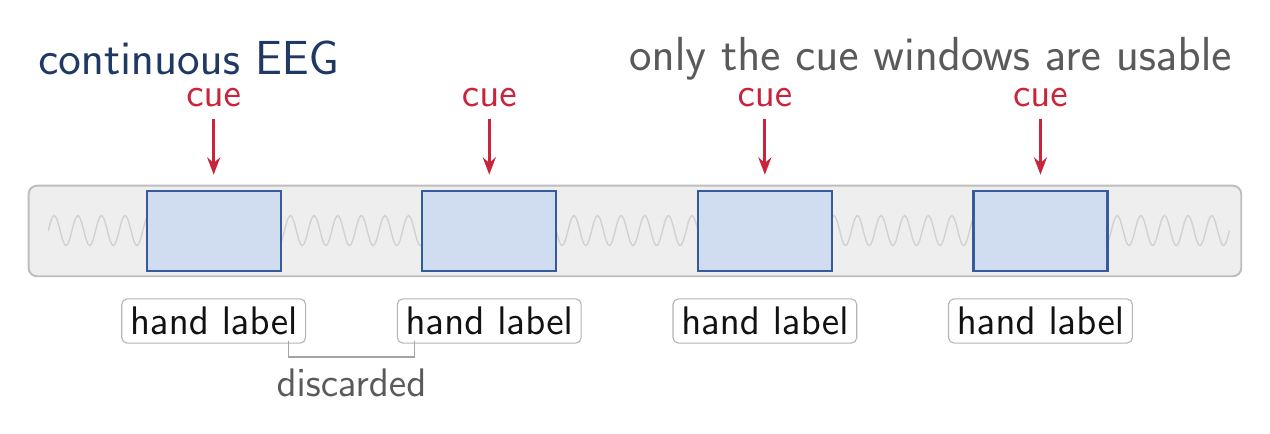
\begin{tikzpicture}[font=\sffamily, >={Stealth[length=2.2mm]}]
  \def\W{15.4}
  \def\H{1.15}

  % the continuous recording
  \fill[otgray!10, rounded corners=3pt] (0,0) rectangle (\W,\H);
  \draw[otgray!40, rounded corners=3pt, line width=0.7pt] (0,0) rectangle (\W,\H);
  \foreach \x in {0.25,0.55,...,15.2}{
    \draw[otgray!28, line width=0.5pt]
      (\x,0.58) sin ++(0.075,0.19) cos ++(0.075,-0.19) sin ++(0.075,-0.19) cos ++(0.075,0.19);}

  % the cue-locked windows that survive
  \foreach \x in {1.5,5.0,8.5,12.0}{
    \fill[otblue!25] (\x,0.07) rectangle ++(1.7,\H-0.14);
    \draw[otblue!80!black, line width=0.8pt] (\x,0.07) rectangle ++(1.7,\H-0.14);
    \draw[otred, line width=1pt, ->] (\x+0.85,\H+0.85) -- (\x+0.85,\H+0.14);
    \node[font=\sffamily\fontsize{15}{17}\selectfont, text=otred, anchor=south]
      at (\x+0.85,\H+0.88) {cue};
    \node[font=\sffamily\fontsize{15}{17}\selectfont, text=otgray!20!black, anchor=north,
          draw=otgray!45, fill=white, rounded corners=2pt, inner sep=3pt]
      at (\x+0.85,-0.28) {hand label};}

  \node[font=\sffamily\fontsize{16}{18}\selectfont, text=otnavy, anchor=west]
    at (0,\H+1.62) {continuous EEG};
  \node[font=\sffamily\fontsize{16}{18}\selectfont, text=otgray, anchor=east]
    at (\W,\H+1.62) {only the cue windows are usable};

  % mark one discarded stretch, clear of the label tags
  \draw[otgray!55, line width=0.7pt] (3.3,-0.82) -- (3.3,-1.02) -- (4.9,-1.02) -- (4.9,-0.82);
  \node[font=\sffamily\fontsize{15}{17}\selectfont, text=otgray, anchor=north]
    at (4.1,-1.05) {discarded};
\end{tikzpicture}
\end{document}
